\chapter{基于内外部知识对齐的检索增强对话生成}

\section{引言}

垂直领域对话生成的一个重要目标就是针对特定领域或行业为用户提供准确、专业、实用的问答服务,基于大型语言模型(LLM)的端到端式对话生成方法是目前实现这一目标的主流方法。LLM在大规模语料上预训练时,广泛的常识知识被内化到模型内部的参数中,成为内部知识,从而使得LLM具有强大的文本理解和生成能力。然而,LLM在生成训练数据之外的垂直领域对话内容时,会出现编造事实的现象,即“幻觉”现象。因此,使用检索增强生成(Retrieval Augmented Generation,RAG)\cite{DBLP:conf/nips/LewisPPPKGKLYR020}技术来提升垂直领域对话生成准确度的做法越来越受到学术界和工业界的关注。

% TODO:研究表明加2篇引用
近年来,大量研究\cite{DBLP:journals/corr/abs-2312-10997}表明,与直接使用LLM生成对话相比,基于检索到的外部知识文档生成的对话内容具备更高的准确性和实时性。然而,基于RAG的垂直领域对话生成方法仍然存在一些局限性。具体而言,LLM在预训练阶段没见过垂直领域的长尾知识,因此检索所补充的外部知识未能与模型内部知识完全对齐,而垂直领域对话涉及到广泛的领域背景知识,知识库检索得到的知识文档不足以覆盖回答用户问题所需的所有前置知识,导致模型无法给出正确的分析和解答。因此,通过对齐LLM内部和外部的知识以提升其生成对话的准确性和相关性是重要且必要的。

采用RAG方法构建外部知识库时,需要从互联网、领域信息平台等来源搜集大量垂直领域知识文档,这些知识文档包含丰富的垂直领域背景知识,可以为LLM内外部知识对齐提供长尾知识训练语料。本章受此启发,提出让LLM从知识库文档中学习垂直领域对话能力,从而解决现有方法的局限。然而,使用外部知识库中的知识文档构建训练数据集用以对齐模型内部知识,具有以下挑战:1)原始知识文档语料质量较低,不适用于对话生成任务;2)不同知识文档之间的知识复杂性不一样,学习难度不同,混合训练导致性能受限;3)推理过程中的检索结果准确度对模型生成效果存在较大影响。

为解决上述挑战,本章提出三点方法。为应对挑战1),本章提出了一种基于多粒度语义切分的指令对生成方法。具体而言,利用基于提示工程的方法或人工标注的方式,从知识文档中分别提取文档级和实体级信息,用以构建数据同分布的外部知识库和监督训练数据集。为克服挑战2),本章提出了一种基于两阶段微调的知识对齐方法。具体而言,将经过多粒度语义切分得到的文档块,按照其任务类别划分为两个数据集,首先在低难度的通用任务数据集上训练,然后在高难度的精标指令数据集上训练,以获得更好的垂直领域对话性能。为解决挑战3),本章提出了一种基于多级混合检索的文档块召回方法。具体而言,首先使用两类不同的检索方法分别对知识库文档块进行排序,然后对二者结果进行融合,最后再对结果进行重排序,以最大程度提升文档块召回准确度。

\section{问题定义}

% 基于大型语言模型的对话生成存在事实性、实时性不足的问题。现有方法主要通过检索增强生成方法进行垂直领域对话生成,以输入的形式将垂直领域知识引入对话模型中。然而,面对垂直领域中较难的问题时,模型往往不能很好理解知识文档中的复杂信息,导致检索增强效果不佳。语言模型在预训练中没见过垂直领域的长尾知识,因此检索增强所补充的知识文档未能与模型内部知识完全对齐。为此,本章研究如何对齐外部知识文档的垂直领域长尾知识和模型内部知识,进而使模型兼具事实性与垂直领域推理能力。同时,本章以金融分析领域为应用场景对算法进行验证。金融分析领域主要涵盖两个关键任务:(1)股票趋势预测任务;(2)金融问答任务。

% 对于股票趋势预测任务,给定一组公司$C=\{c_i\}_{i=1}^N$以及对应的知识文档$D=\{d_j\}_{j=1}^M$,对话系统给出该股票的未来趋势预测:
% \begin{equation}
% 	Pred_i=\pi(c_i, d_j), Pred_i \in \{up, down\}
% \end{equation}
% 其中,$\pi$表示对话系统,$d_j$是检索得到的与公司$c_i$相关的知识文档。目标是选择出一批被预测股价会上涨的公司:
% \begin{equation}
% 	C_{chosen} = \{c_i | c_i \in C \land Pred_i = up\}
% \end{equation}
% 目前机器学习和深度学习的方法已经被广泛应用在该任务上,并取得了一定的进展\cite{RJXB20240320003,RJXB201903021}。然而,这些方法通常只能基于过去的市场价格数据预测未来股票的涨跌,而无法给出具体的分析过程和原因,其预测结果对投资者用户来说缺乏可解释性。同时,这类方法难以将新闻、研报等非结构化的文本信息用于股票趋势预测中。

% 对于金融问答任务,本章将一个多轮对话视为两个对话者之间的诸多“问题-回复”对。令$Q_t$和$R_t$表示在第$t$轮对话时的用户问题和系统回复,$H_t=[Q_0, R_0, …, Q_{t-1}, R_{t-1}]$作为对话历史。本章将金融问答任务的形式定义为,给定对话历史、用户问题和检索到的相关文档,对话系统$\pi$能够给出相应的回复:
% \begin{equation}
% 	R_t = \pi(d_k, H_t, Q_t)
% \end{equation}
% 其中,$d_k$表示检索到的与$Q_t$相关的知识文档。
% 目前大部分的金融问答方法主要基于大型语言模型,这类模型在大规模语料上经过预训练,具有强大的文本理解和文本生成能力。但由于金融领域数据集的稀缺性和模型微调的知识滞后性,语言模型存在不可控的“幻觉”问题,即编造没有现实基础的事实或细节。因此,一些基于检索增强生成的方法提出利用知识库检索出与用户问题相关的外部知识辅助模型生成回答,一定程度上缓解了大型语言模型的幻觉问题和实时性问题。然而,对于某些金融领域问题,涉及到广泛的金融背景知识,仅依靠知识库检索得到的知识文档并不足以让模型给出正确的分析和解答。

面向垂直领域的检索增强对话生成任务要求对话系统根据给定的垂直领域用户问题,结合相关外部知识进行专业性的回复生成。将一个多轮对话视为两个对话者之间的诸多“问题-回复”对,给定在第$t$轮对话时的用户问题$Q_t$和对话历史$H_t=[Q_0, R_0, …, Q_{t-1}, R_{t-1}]$,在外部知识库中检索与$Q_t$相关的知识文档$d_k$,对话系统利用$Q_t$、$H_t$和$d_k$输出准确的分析与解答回复$R_t$。

\section{本章方法}
\subsection{算法总体框架}

\begin{figure}[htbp]
	\centering
	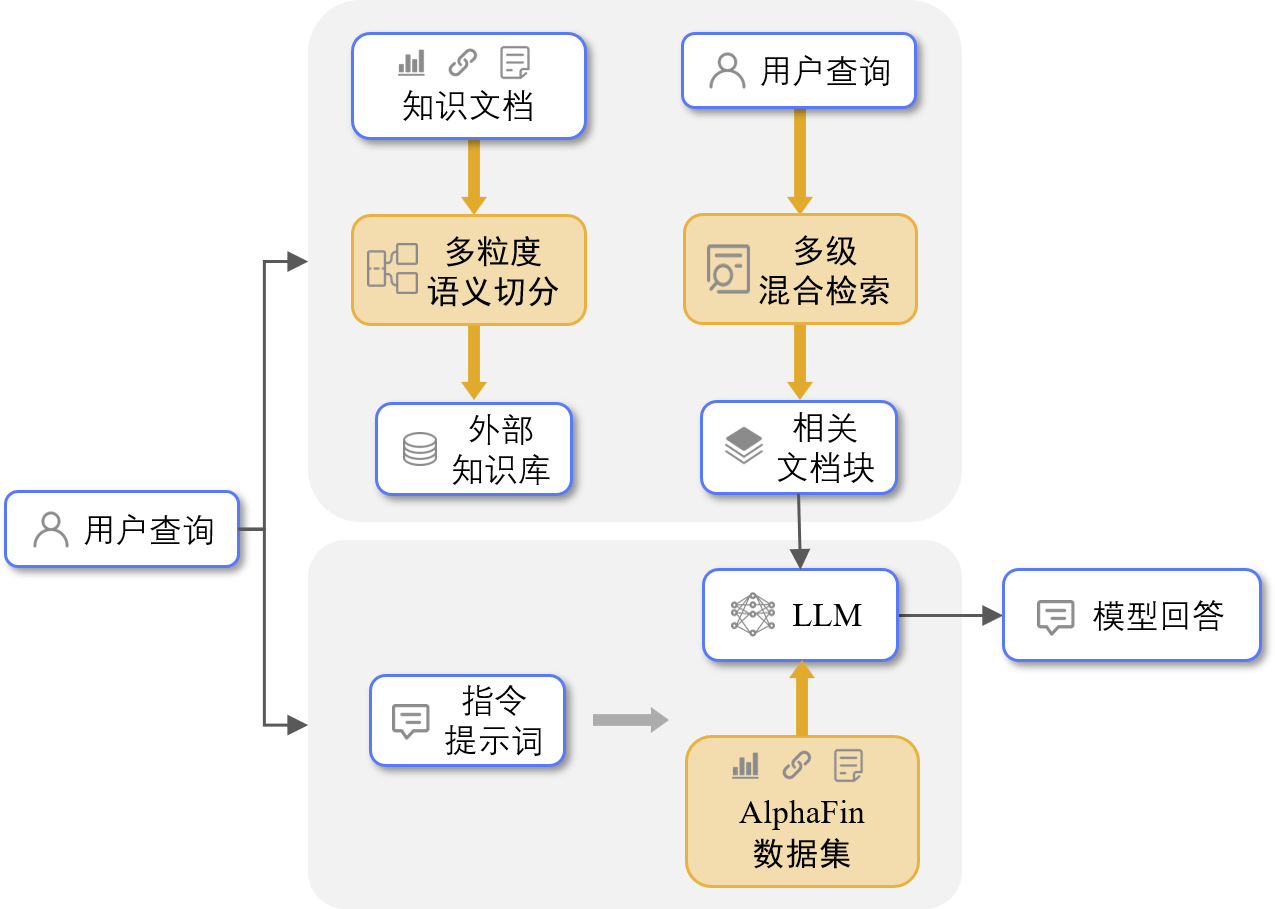
\includegraphics[scale=0.65]{Fig/rag_framework.png}
	\caption{\label{rag_framework}本章所提出的检索增强对话生成框架示意图。}
\end{figure}

针对以上问题,本章提出基于内外部知识对齐的检索增强对话生成方法。整体算法框架如图\ref{rag_framework}所示,整个框架主要包括三个部分:(1)对垂直领域知识文档进行多粒度语义切分,得到一系列垂直领域知识文档块,并构建外部知识库用于存储和检索这些知识文档块;(2)构建垂直领域数据集,为模型注入垂直领域的内部知识,同时与知识库中的外部知识进行对齐;(3)利用多级混合检索,对用户问题和知识库中的文档块计算语义相似度,得到与用户问题相关性最高的一系列文档块,最后与指令提示词拼接输入模型,得到回答。

\subsection{基于多粒度语义切分的指令对生成}

\begin{figure}[htbp]
	\centering
	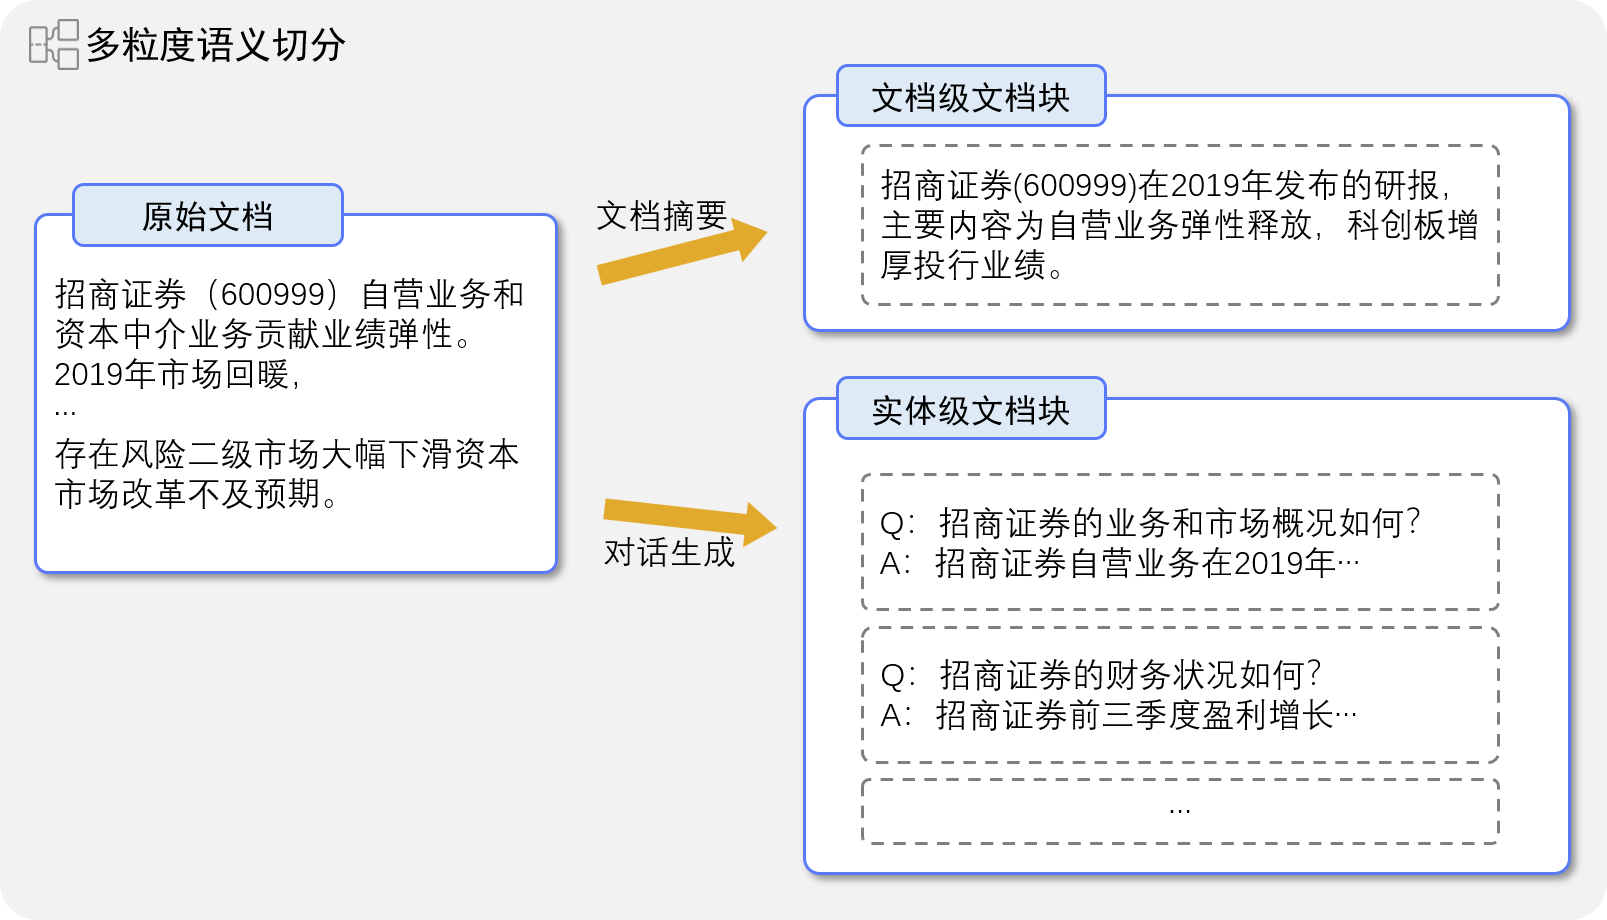
\includegraphics[scale=0.5]{Fig/split_chunk_module.png}
	\caption{\label{split_chunk_module}对话框架中的多粒度语义切分模块示意图。}
\end{figure}

外部知识库的构建是检索增强生成中的的重要组成部分,用于高效存储和检索相关知识文档。外部知识是指显式存储在外部知识库中的知识,内部知识是指通过模型训练隐式存储在神经网络权重中的知识,二者的数据来源和数据分布存在差异,导致检索增强对话生成存在性能瓶颈。为了实现外部知识与模型内部知识的对齐,本节提出一种基于多粒度语义切分的指令对生成方法,从文档中提取出关键信息,构成指令对数据,用于外部知识库和监督微调数据集的构建。如图\ref{split_chunk_module}所示,本章采用两种切分策略:粗粒度文档级总结和细粒度实体级Q\&A对生成。其中,语义切分过程由垂直领域人类专家编写,或使用LLM(如ChatGPT模型)通过设计相应的提示词完成,本章所使用的语义切分提示词如表\ref{gen_finqa_prompt}所示。

\begin{table}
	\caption{\label{gen_finqa_prompt}知识文档语义切分提示词。}
	\centering{}%
	\small 
	\begin{tabular}{c}
		\toprule[2pt]
		提示词\tabularnewline
		\hline 
		\begin{tabular}{l}
			基于<content>,请提出一个<domain>领域的专业问题。 \\ 输入:<sequential data> \\ 输出:<question>
		\end{tabular} \\
		\bottomrule[2pt]
	\end{tabular}
\end{table}

对于文档$d_k$,其语义切分过程如下:
\begin{equation}
	s_k = LLM_{sum}(d_k)
\end{equation}
\begin{equation}
	(q_{k0}, a_{k0}), (q_{k1}, a_{k1}), \dots = LLM_{qa}(d_k)
\end{equation}
其中,$s_k$表示文档$d_k$的摘要,$(q_{k\_}, a_{k\_})$是所生成对话的“问题-回答”二元组。例如,以医疗领域为例,假设$d_k$是与“核磁共振”相关的文档,$q_{k\_}$则可能是“如何根据核磁共振报告了解具体病情?”。

\subsection{基于两阶段微调的知识对齐}

本节构建了垂直领域监督训练数据集用于微调对话模型,以弥合内外部知识之间的分布差异,从而提升语言模型在垂直领域知识密集型对话任务上的性能。本节所构建的监督微调数据集包含两个部分:1)通用任务数据集,由较低难度的通用任务指令对数据构成,包含情感分析、命名实体识别、文本分类、文本摘要等传统NLP任务,样本输出长度在100个标识符以内;2)精标指令数据集,由较高难度的逻辑推理、知识问答指令对数据构成,样本输出长度在100个标识符以上。

模型微调过程分为两个阶段:1)首先在通用任务数据集上进行自回归训练,目的是将专业领域的基本知识注入模型内部;2)然后,在上一步微调后的模型基础上进行继续训练,以进一步对齐知识文档中的长尾知识与模型内部的知识,同时使模型学会复杂任务的输出格式。所有的微调过程均采用LoRA方法,以缓解训练过拟合问题,同时降低训练成本。微调后的模型将作为对话框架中的对话生成模型,与用户交互。

\subsection{基于多级混合检索的文档块召回}

\begin{figure}[htbp]
	\centering
	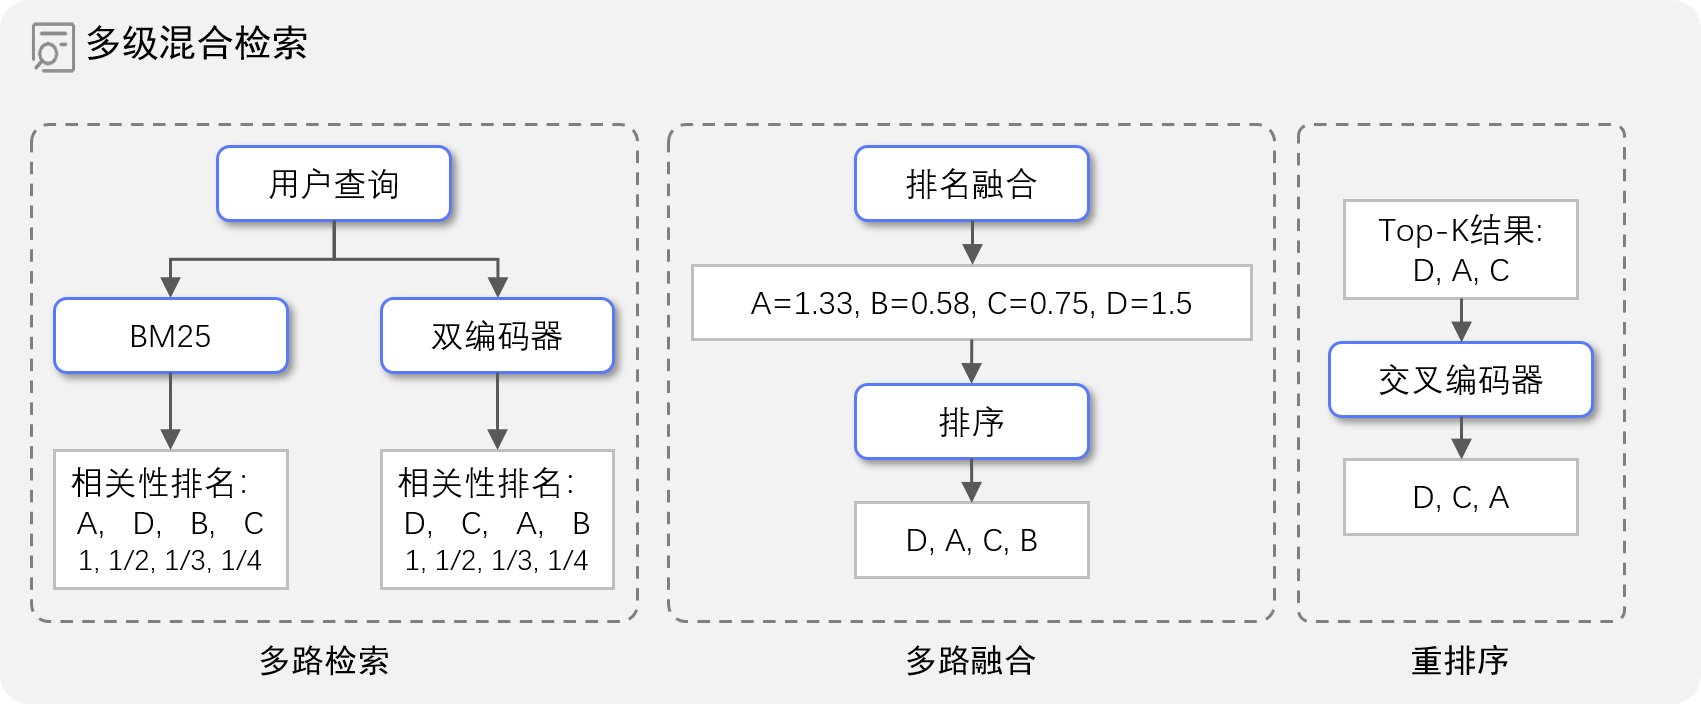
\includegraphics[scale=0.55]{Fig/search_module.png}
	\caption{\label{search_module}对话框架中的多级混合检索模块示意图。}
\end{figure}

如图\ref{search_module}所示,多级混合检索模块主要包含三个步骤:(1)多路检索;(2)多路融合;(3)重排序。本节以文档级摘要切分策略为例,说明多级混合检索的具体计算过程。其中,对于细粒度实体级对话生成的切分策略,下式中的$s_k$和$d_k$可分别被替换为$q_{k\_}$和$a_{k\_}$。

\textbf{多路检索} 本节使用稀疏向量检索和稠密向量检索两种方式。BM25算法是常用的稀疏向量检索算法,通过词频逆文档频率(TF-IDF)计算用户问题和知识文档的词汇重叠率,从而得到二者的相似度得分。相较于稠密向量检索,BM25算法能够较好地从通用实体泛化到垂直领域罕见实体,缓解长尾效应。同时,BM25算法能够考虑到词在文档中的分布情况,更好的捕捉到词的上下文信息。给定用户问题$Q$和文档摘要$s_k$,其BM25相似度评分计算过程如下:
\begin{equation}
	Score_{bm25}(Q, s_k) = \sum_{i}^{N}IDF(q_i, s_k)\frac{f_i(k_1+1)}{f_i + k_1(1 - b + b\frac{sl}{avg(sl)})}
\end{equation}
\begin{equation}
	IDF(q_i, s_k) = log\frac{sl-n_i+0.5}{n_i+0.5}
\end{equation}
其中,$N$表示$Q$中的单词数量,$q_i$表示$Q$中的第$i$个单词,$k_1$、$k_2$和$b$是调节因子,本节分别设置为2、0、0.75。$f_i$表示单词$q_i$在文档$s_k$中出现的频率,$n_i$表示$q_i$在$s_k$出现的次数,$sl$为文档$s_k$的长度,$avg(sl)$为知识库中所有文档的平均长度。基于评分$Score_{bm25}$对所有文档进行排序,可得到文档排列$R_{bm25}$。

然而,BM25存在数据稀疏问题,导致文档中的重要信息被忽略。基于双编码器(Bi-Encoder)的稠密向量检索方法能将文本映射为词嵌入向量,对目标词及其上下文进行建模,更好的捕捉到文本的语义信息,使得语义向量能够更好地表示用户问题的意图,获得更准确和全面的检索结果。因此本章同时还使用了基于双编码器的稠密检索方法,与稀疏检索互为补充。

给定用户问题$Q$和文档摘要$s_k$,分别通过双编码器模型得到对应的嵌入向量$e_Q$和$e_{sk}$。所有文档的嵌入向量$e_{sk}$将被存储在知识库中,作为数据库索引被用于后续的检索步骤。
\begin{equation}
	e_{sk} = BE(s_k)
\end{equation}
\begin{equation}
	e_Q = BE(Q)
\end{equation}
其中,$BE$是双编码器模型,如BGE\cite{DBLP:journals/corr/abs-2309-07597}、SGPT\cite{DBLP:journals/corr/abs-2202-08904}等。基于评分$Score_{emb}$对所有文档进行排序,可得到文档排列$R_{emb}$。

\textbf{多路融合} 由于不同检索方式使用的相关度评分存在量纲差异,因此不宜直接对多路检索评分结果求和。本节使用排名融合方法,对文档排列$R_{bm25}$和$R_{emb}$进行合并。文档摘要$s_k$的排名融合评分计算过程如下:
\begin{equation}
	Score_{RRF} = \sum_{r \in \{R_{bm25},R_{emb}\}}\frac{1}{k + r(s_k)}
\end{equation}
其中,$k$为超参数,本节设置为60。基于排名融合评分重新排序,得到文档排列$R_{RRF}$。

\textbf{重排序} 交叉编码器计算速度慢,且无法预先计算文本嵌入向量,只能实时计算文本对的语义相似度分数,但是其准确度优于双编码器,因此适用于对双编码器结果的检索结果进行二次精排。本节选取多路融合结果的Top-K文档排列,分别与用户问题一起输入交叉编码器,得到语义相似度分数,选择相似度分数最高的文档作为最终的结果$d^*$。
\begin{equation}
	d^* = \mathop{\arg\max}_{d_k}CE(s_k), \quad s_k \in topk(R_{RRF})
\end{equation}
其中,$CE$表示交叉编码器模型,$topk(\cdot)$表示取排列中的前k个元素。

\subsection{回答生成}

给定对话历史$H_t$,用户问题$Q_t$,以及检索到的与用户问题$Q_t$相关的文档$d^*$,目标是获得第$t$轮对话的回复$R_t$。然后,拼接提示词模板、知识文档、对话历史和用户问题,以得到LLM的输入$I_t$。将$I_t$传入LLM,即可得到回复$R_t$。
\begin{equation}
	I_t = concat(Prompt, d^*, H_t, Q_t)
\end{equation}
\begin{equation}
	R_t = LLM(I_t)
\end{equation}

\section{实验结果}

本节以金融领域为应用场景对算法进行实验验证。金融领域分析任务主要包括两个部分:1)股票趋势预测;2)金融问答。对于第一类任务,主要考察模型的对股票相关信息的理解能力和趋势预测能力,通过年化收益率和预测准确率体现。对于第二类任务,主要考察模型对用户问题解答的准确性、相关性、和有帮助性,通过人工偏好评价和GPT-4偏好评价体现。

\subsection{数据集介绍}

为说明本章方法在金融分析领域的有效性,本章在两个基准测试集上进行实验,即AlphaFin-test和FinGPT-FiQA\cite{wang2023fingptbenchmark}。两个数据集都包含金融领域对话数据。其中,在股票涨跌预测任务上,本节使用AlphaFin-test测试集中的金融研报数据集进行实验;在金融问答任务上,为保证样本数据分布的广泛性,本节同时使用AlphaFin-test的金融新闻\&问答数据集、AlphaFin-test的金融研报数据集和FinGPT-FiQA三个测试集进行实验。同时,由于金融问答任务实验使用人工和GPT-4模型进行评估,评估成本较高,本实验对所有基准测试集均随机抽取1000个样本进行实验。

\begin{itemize}[topsep = 0 pt, itemsep= 0 pt, parsep=0pt, partopsep=0pt, leftmargin=36pt, itemindent=0pt, labelsep=6pt, listparindent=24pt]
	\item FinGPT-FiQA:FinGPT-FiQA包含171000个金融领域英文指令问答样本,每个样本包含系统指令、输入、输出三个字段。输入字段为金融领域的问题或话题,输出为针对输入的回答或观点,所有样本均为单轮对话。

	\item AlphaFin-test:AlphaFin-test是从本章所提出的AlphaFin数据集中划分出来的测试集,与AlphaFin训练集没有交集。AlphaFin-test为中文数据集,包含金融新闻\&问答数据集和金融研报数据集两个部分。金融新闻\&问答数据集有10000个样本,每个样本包含系统指令、输入和输出字段,包含针对金融新闻、金融数据的单轮问答对话。金融研报数据集有1000个样本,涵盖544家上市公司在2020年1月到2023年7月的真实市场数据,每个样本包含系统指令、输入和输出三个字段,在输入字段中给出指定公司在指定日期的研报和当月股价数据,在系统指令中要求给出该公司股票次月涨跌分析及预测,输出字段为该股票的实际涨跌结果。
\end{itemize}

接下来详细介绍AlphaFin数据集的具体构建方式及具体信息。如图\ref{dataset_process}所示,AlphaFin数据集包含三部分:通用金融数据集、金融新闻与问答数据集、金融研报数据集。其中,通用金融数据集作为本章的通用任务数据集,其余两个数据集作为本章的精标指令数据集。各数据集具体来源和预处理方式如下:

\begin{figure}[htbp]
	\centering
	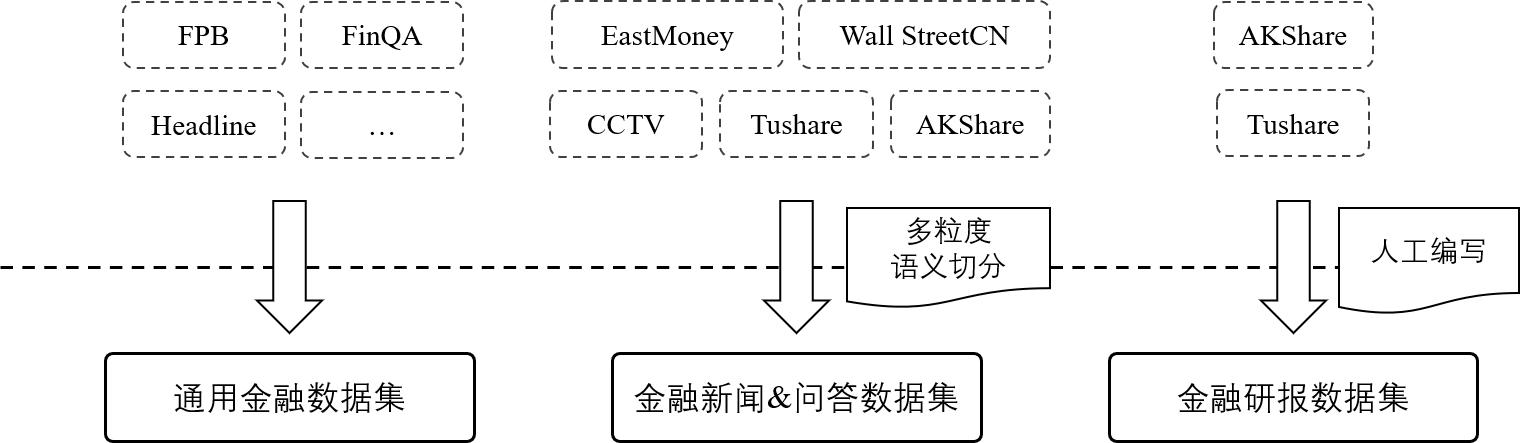
\includegraphics[scale=0.6]{Fig/dataset_process.png}
	\caption{\label{dataset_process}数据集预处理过程示意图。}
\end{figure}

\textbf{通用金融数据集} 由传统金融开源数据集构成,如FPB\cite{DBLP:journals/jasis/MaloSKWT14}、FinQA\cite{DBLP:conf/acl/ZhuLHWZLFC20}、ConvFinQA\cite{DBLP:journals/corr/abs-2310-00566}、Headline\cite{DBLP:journals/corr/abs-2009-04202}等,涵盖情感分析、文本摘要等基础NLP任务。这些开源数据集均为英文数据集,因此本节从中采样一部分,用于增强模型的多语言能力、信息抽取能力和摘要能力。

\textbf{金融新闻数据集} 爬取自互联网媒体发布的财经新闻稿件,如CCTV金融板块、华尔街见闻等。利用ChatGPT\cite{DBLP:conf/nips/Ouyang0JAWMZASR22}模型进行多粒度语义切分,对每条新闻分别提取出文档级摘要和实体级对话,构成金融新闻数据集。该数据集用于增强模型对金融新闻的理解能力与摘要能力。

\textbf{金融问答数据集} 爬取自开源金融数据接口库,如Tushare\cite{tushare}、AKshare\cite{akshare}等。该部分主要包含股票价格及其他财务信息的时序数据(例如[‘2023-10-02’: 172.40…‘2023-10-12’: 180.71, …]),然后基于多粒度语义分割模块,得到与数据相关的金融问答数据,如“根据如下资产负债表数据...,请计算出该公司的流动比率是多少?”。该数据集用于增强模型的数学逻辑能力。

\begin{table}
	\caption{\label{financial_report_format}金融研报数据集样本格式。}
	\centering
	\begin{tabular}{c|c|c}
		\toprule[2pt]
		数据集 & Raw类型 & CoT类型 \\
		\hline
		系统指令 & \multicolumn{2}{l}{
			\begin{tabular}{p{12cm}}
				请根据下方提供的该股票相关研报与数据,对该股票的下个月的涨跌,进行预测,请给出明确的答案,“涨” 或者 “跌“。同时给出这个股票下月的涨跌概率,分别是:极大,较大,中上,一般。\\
			\end{tabular}
		} \\
		\hline
		输入 & \multicolumn{2}{l}{
			\begin{tabular}{p{12cm}}
				<|公司研报|> \\ 发布日期:<date> \\ 研报题目:<title> \\ 目标价格:<target price> \\ 研报摘要:<abstract> \\  \\ <|市场数据|> \\ 1.股票价格(元):<price>; \\ 2.日涨跌幅(\%):<change>; \\ 3.日成交量(亿):<volumn> \\
			\end{tabular}
		} \\
		\hline
		输出 & 
		\begin{tabular}{p{3.8cm}}
			这个股票的下月最终收益结果是:'跌',下跌概率:中上 \\
		\end{tabular} & 
		\begin{tabular}{p{8.2cm}}
			通过公司研报和市场数据可以得出以下结论: \\ 1、基本面: <basic analysis>。 \\ 2、技术面: <tech analysis>。 \\ 因此,我们预测,这个股票的下月最终收益结果是:'跌',下跌概率:极大 \\
		\end{tabular} \\
		\bottomrule[2pt]
	\end{tabular}
\end{table}

\textbf{金融研报数据集} 分别从DataYes数据平台接口和TuShare、AKShare接口爬取股票研究报告和股票价格时序数据,股票研究报告包括证券公司对上市公司的专业分析。本节人工对齐公司的研究报告及其在报告发布当天的股票价格,并使用如表\ref{financial_report_format}所示的格式来构建样本输入部分,将股票在报告发布次月的真实股价涨跌情况作为样本输出。其中,金融研报数据集包含两种类型的数据:1)Raw类型,样本输出中仅包含股票涨跌结果和涨跌概率;2)CoT类型,在给出股票涨跌预测结果前,先对输入中的公司研报和市场数据信息进行基本面和技术面的详细分析和逻辑推导,作为模型推理思维链,这部分CoT分析由金融领域专家人工编写,以保证其正确性和质量。该数据集用于增强模型的金融分析能力,让模型学习金融分析的格式。

\begin{table}
	\caption{\label{alphafin_info}AlphaFin数据集统计信息。}
	\centering
	\begin{tabular}{lccccc}
		\toprule[2pt]
		数据集 & 类别 & 大小 & 输入长度 & 输出长度 & 语言 \\
		\hline
		通用金融数据集 & - & 42,373 & 712.8 & 5.6 & 英文 \\
		\hline
		\multirow{2}*{金融新闻\&问答数据集} & 新闻 & 21,000 & 1313.6 & 40.8 & 中文 \\
		~ & 问答 & 79,000 & 497.8 & 64.2 & 中文 \\
		\hline
		\multirow{2}*{金融研报数据集} & Raw & 120,000 & 2203.0 & 17.2 & 中文 \\
		~ & CoT & 200 & 2184.8 & 407.8 & 中文 \\
		\bottomrule[2pt]
	\end{tabular}
\end{table}

最终得到的AlphaFin数据集各组成部分的统计信息如表\ref{alphafin_info}所示,任务类型涵盖NLP基础任务、金融新闻、金融问答、研报分析,不同任务类型、不同语言的数据量相当,以保证模型学习到的各项能力趋于平衡。

\subsection{基准方法}

\begin{itemize}[topsep = 0 pt, itemsep= 0 pt, parsep=0pt, partopsep=0pt, leftmargin=36pt, itemindent=0pt, labelsep=6pt, listparindent=24pt]
	\item 股票指数:本节选取了中国股票市场的重要指数,包括上证50、沪深300、上证指数和创业板指数。这类指数反映了某个交易板块中所有上市公司股票的整体涨跌情况,即市场综合水平。
	\item 机器学习模型:随机森林\cite{DBLP:journals/pami/Ho98}、RNN\cite{rumelhart1986learning}、BERT\cite{DBLP:conf/naacl/DevlinCLT19}、GRU\cite{DBLP:conf/emnlp/ChoMGBBSB14}、LSTM\cite{DBLP:journals/neco/HochreiterS97}、逻辑回归\cite{cox1958regression}、XGBoost\cite{DBLP:conf/kdd/ChenG16}、决策树\cite{DBLP:books/mk/Quinlan93}等。
	\item LLM:包含ChatGLM2-6B\cite{DBLP:conf/iclr/ZengLDWL0YXZXTM23}和ChatGPT\cite{DBLP:conf/nips/Ouyang0JAWMZASR22},在通用任务上进行监督微调,具有对话能力的LLM。
	\item 金融LLM:包含FinMA\cite{DBLP:journals/corr/abs-2306-05443}和FinGPT\cite{DBLP:journals/corr/abs-2306-06031},在金融领域数据集上微调后的LLM,能够处理广泛的金融任务。
\end{itemize}

% \begin{itemize}[topsep = 0 pt, itemsep= 0 pt, parsep=0pt, partopsep=0pt, leftmargin=36pt, itemindent=0pt, labelsep=6pt, listparindent=24pt]
% 	\item 股票指数:本节选取了中国股票市场的重要指数,包括上证50(SSE50)、沪深300(CSI300)、上证指数(SCI)和创业板指数(CNX)。这类指数反映了某个交易板块中所有上市公司股票的整体涨跌情况,即市场综合水平,因此本节使用这类股票指数作为市场基本走势的参考。
% 	\item 随机森林\cite{DBLP:journals/pami/Ho98}:随机森林是一种监督式学习算法,主要用于分类和回归问题,它是由多个决策树组成的集成模型。其核心思路是,当训练数据被输入模型时,采用不同的子集和特征属性分别建立多个小的决策树,然后将它们集成为一个更强大的模型,而非用整个训练数据集建立单个大的决策树。
% 	\item RNN\cite{rumelhart1986learning}:循环神经网络(Recurrent Neural Network,简称RNN)是一种特殊的神经网络,它能够处理序列数据,并利用序列中的历史信息进行学习。RNN的结构包含一个循环单元,这个单元允许信息在时间步骤之间传递,使得网络能够记忆和处理之前时刻的信息。
% 	\item BERT\cite{DBLP:conf/naacl/DevlinCLT19}:BERT是一种语言表示模型,BERT代表来自Transformer的双向编码器表示(Bidirectional Encoder Representations from Transformers)。BERT旨在通过联合调节所有层中的双向上下文来预训练深度双向表示。因此适用于文本理解、机器翻译等任务。
% 	\item GRU\cite{DBLP:conf/emnlp/ChoMGBBSB14}:GRU(Gated Recurrent Unit)是一种门控循环单元,属于循环神经网络(RNN)的一种。它的主要特点是具有两个门:更新门(update gate)和重置门(reset gate)。更新门负责控制上一时刻状态信息对当前时刻状态的影响,而重置门负责控制忽略前一时刻的状态信息的程度。GRU是一种简单而有效的RNN变体,它在保持与LSTM相当性能的同时,减少了参数数量,提高了训练效率,因此在实际应用中常常被优先选择。
% 	\item LSTM\cite{DBLP:journals/neco/HochreiterS97}:LSTM(Long Short-Term Memory)是一种特殊的循环神经网络(RNN),它能够有效地捕捉和记忆长序列中的信息,克服了传统RNN中梯度消失或爆炸的问题。LSTM的核心结构包括四个部分:遗忘门、输入门、细胞状态和输出门。它通过门控机制控制信息的流动,从而在序列学习中表现出强大的能力。
% 	\item 逻辑回归\cite{cox1958regression}:逻辑回归是一种统计学习方法主要用于二分类问题,即输出只有两种,分别代表两个类别。逻辑回归的优点包括速度快,适合二分类问题,简单易于理解,直接看到各个特征的权重,能容易地更新模型吸收新的数据。
% 	\item XGBoost\cite{DBLP:conf/kdd/ChenG16}:XGBoost是一个优化的分布式梯度增强库,旨在实现高效,灵活和便携。它在 Gradient Boosting 框架下实现机器学习算法。XGBoost提供并行树提升(也称为GBDT,GBM),可以快速准确地解决许多数据科学问题。
% 	\item 决策树\cite{DBLP:books/mk/Quinlan93}:决策树是一种树形结构,用于分类和回归问题,它通过一系列的判断(节点)和决策(边)来预测实例的类别。决策树的特点包括计算复杂度不高、输出结果易于理解、对中间值的缺失不敏感,可以处理不相关特征数据。此外,决策树是一种非参数的有监督学习方法,它能够从一系列有特征有标签的数据中总结出决策规则并用树状图的结构来呈现这些规则。
% 	\item ChatGLM2-6B\cite{DBLP:conf/iclr/ZengLDWL0YXZXTM23}:ChatGLM2-6B是中英双语对话模型。它使用了 GLM 的混合目标函数,经过了1.4T中英文标识符的预训练,在CEval、GSM8K等数据集上得到大幅度的性能提升。
% 	\item ChatGPT\cite{DBLP:conf/nips/Ouyang0JAWMZASR22}:ChatGPT是基于GPT(Generative Pre-trained Transformer)架构的闭源大型语言模型,它基于RLHF算法进行人类偏好反馈对齐训练,具有良好的对话生成能力。
% 	\item FinMA\cite{DBLP:journals/corr/abs-2306-05443}:FinMA是一个综合性金融大型语言模型(LLM)。它旨在理解复杂的金融语言和概念,并经过微调以遵循自然语言指令,提高其在下游金融任务中的性能。它使用自建金融数据集的完整指令数据进行训练,涵盖了NLP和预测任务。这使它成为一种更全面的模式,能够处理更广泛的金融任务。
% 	\item FinGPT\cite{DBLP:journals/corr/abs-2306-06031}:FinGPT是面向金融领域的大型语言模型系列。它使用自建金融数据集在LLaMA2-13B\cite{DBLP:journals/corr/abs-2307-09288}、ChatGLM2-6B等预训练模型上进行LoRA微调,得到金融领域语言模型。本实验所使用的是基于ChatGLM2-6B的版本。
% \end{itemize}

\subsection{评价指标}

对于股票趋势预测任务,本节使用两类指标。第一类是核心指标,包括衡量收益能力的年化收益率(ARR)和准确率(ACC)。第二类是辅助分析的观察指标,如最大回撤(MD),卡玛比率(CR),夏普比率(SR),用于评估投资组合风险情况。具体介绍如下。

\begin{itemize}[topsep = 0 pt, itemsep= 0 pt, parsep=0pt, partopsep=0pt, leftmargin=36pt, itemindent=0pt, labelsep=6pt, listparindent=24pt]
	\item 年化收益率(ARR):将当前收益率按照复利计算(即每年收益计入本金),折算成平均年度收益率。其计算公式为:$ARR = (Return / Principle)^{1/n} - 1$,其中$n$为投资年数,$Return$为总收益,$Principle$为本金。
	\item 准确率(ACC):当模型对股票涨跌预测结果与次月实际涨跌趋势一致时,可认为模型预测正确(ACC=1),否则预测错误(ACC=0)。
	\item 年化超额收益率(AERR):投资组合的ARR超过基准ARR的部分,即$AERR = ARR - ARR_{b}$,本实验中$ARR_{b}$取沪深300的ARR。
	\item 年化波动(ANVOL):用于衡量投资组合的波动风险,其计算公式为:$ANVOL = \sigma_P * \sqrt{n}$,其中$\sigma_P$为收益率标准差,$n$为投资年数。
	\item 最大回撤(MD):在选定周期内任一时间点开始,产品净值下降到最低点时的收益率最大回撤幅度,用于表现投资组合可能出现的最糟糕情况。其计算公式为:$MD = max((D_i - D_j) / D_i)$,$D_i$表示第$i$天的资产净值,且$i < j$。
	\item 卡玛比率(CR):表示投资组合收益和最大回撤之间的关系,代表每单位回撤能获得的收益率。其计算公式为:$CR = ARR / MD$。
	\item 夏普比率(SR):投资组合每承受一单位总风险,所产生的超额收益。其计算公式为:$SharpRatio = (E(ARR) - R_f)/\sigma_P$,其中$E(ARR)$表示投资组合的ARR期望,$R_f$为年化无风险利率,$\sigma_P$为投资组合收益率的标准差。
	\item 最大下潜期(MDD):描述持有价值从回撤开始到再创新高所经历的时间,该指标可以反映资产创新高的频率。
\end{itemize}

对于金融问答任务,本节使用ROUGE作为评价指标,用于衡量生成的输出和参考信息之间的相似性。此外,本节还使用人工与GPT-4作为评判员,对模型回复进行两两配对评估。同时,本节还使用Ragas\cite{DBLP:conf/eacl/ESJAS24}检索增强评估框架中的context\_precision、context\_recall、faithfulness三项指标对本章方法进行评估。指标具体介绍如下。

\begin{itemize}[topsep = 0 pt, itemsep= 0 pt, parsep=0pt, partopsep=0pt, leftmargin=36pt, itemindent=0pt, labelsep=6pt, listparindent=24pt]
	\item ROUGE:机器翻译、文本摘要等自然语言处理任务中的常用评估指标,基于模型生成的候选值和参考答案计算其N-gram召回率。其中,ROUGE-L计算的是二者的最长公共子序列长度。
	\item 人类偏好评价:由人类担任评判员,从两个不同模型的回复中选择更优的回答,考察角度包括回答的有帮助性、相关性、准确性、深度、创造性和详细程度。
	\item GPT-4偏好评价:由GPT-4\cite{DBLP:journals/corr/abs-2303-08774}模型担任评判员,从两个不同模型的回复中选择更优的回答,考察角度与人类偏好评价保持一致,并在系统指令中对GPT-4模型进行约束,指令提示词格式参考MT-Bench\cite{zheng2023judging}评估框架。
	\item 上下文准确率(Context Precision):利用LLM(如GPT-4模型)评估知识文档块与用户问题之间的相关性及文档块排名顺序。
	\item 上下文召回率(Context Recall):利用LLM估计模型回答和文档块的TP和FN,计算文档块的召回率。
	\item 可信度(Faithfulness):利用LLM计算(用户问题, 模型回答, 文档块)三元组的自然语言推断(NLI)分数,即对模型回答的事实性进行量化评估。
\end{itemize}

\subsection{实验细节}

\begin{table}
	\caption{\label{env_setting}实验环境配置参数。}
	\centering
	\begin{tabular}{ccc}
		\toprule[2pt]
		实验环境 & 配置 & 具体参数 \\
		\hline
		\multirow{2}*{硬件环境} & GPU & NVIDIA A800-SXM4-80GB$\times$1 \\
		~ & 内存 & 128GB \\
		\hline
		\multirow{5}*{软件环境} & 深度学习框架 & PyTorch 1.12.1 \\
		~ & 开发语言 & Python 3.8.13 \\
		~ & 开发工具 & Visual Studio Code \\
		~ & \multirow{2}*{其他重要依赖库} & peft 0.5.0 \\
		~ & ~ & transformers 4.33.0 \\
		\bottomrule[2pt]
	\end{tabular}
\end{table}
本节实验中所有语言模型的推理解码策略均为贪心搜索,以达到最稳定的性能。另外,在所有模型训练过程中,所使用的超参数如下:Batch Size=16,LoRA Rank=8,学习率调度器为CosineLRScheduler,Learning Rate=5e-5,Precision=bf16,其余硬件和软件环境如表\ref{env_setting}所示。其中,在股票趋势预测任务中,模型在AlphaFin金融研报数据集上训练了20个epoch。在金融问答任务中,使用股票趋势预测中的模型作为基础模型,并在AlphaFin金融新闻\&问答数据集上对其进行2个epoch的增量微调。

同时,对于股票趋势预测任务,为观察模型在真实市场中的模拟投资表现,本节采用如下处理方法进行投资策略生成:

给定输入$I_i$,本节利用LLM来预测股票的涨跌趋势,这可以看作是一个二分类任务。通过将$I_i$输入LLM,得到关于$c_i$的回复文本$Res_i$。
% \begin{equation}
% 	Res_i = LLM(I_i)
% \end{equation}

然后,使用基于规则的方法从$Res_i$中提取出趋势预测结果$Pred_i$,选择所有被预测为“上涨”的股票,得到股票集合$C_chosen$。
\begin{equation}
    Pred_i = \left\{ 
        \begin{array}{ll}
            up, & if\ \ ``up" \in Res_i \\
            down, & else \\
        \end{array}
    \right.
\end{equation}
\begin{equation}
	C_{chosen}= \{c_i | Pred_i = up\}
\end{equation}

最后,本节按月滚动执行该投资策略。即,在每个月月初买入或继续持有$C_{chosen}$中的所有股票$c_i$,持有时间为一个月。投资组合中的每种股票的比例是通过市值加权计算得到的。
\begin{equation}
	AR_m = AR_{m-1} + \sum_{c_i \in C_{chosen}}\omega_{c_i} R_{c_i}
\end{equation}
其中,$AR_m$表示第$m$个月的累计收益,$R_{c_i}$表示股票$c_i$的收益。$\omega_{c_i}$代表股票$c_i$在投资组合中所占的比例。$v_i$是公司$c_i$的市值。
\begin{equation}
	\omega_{c_i} = \frac{v_i}{\sum_{c_n \in C_{chosen}}v_n}
\end{equation}

\begin{figure}[htbp]
	\centering
	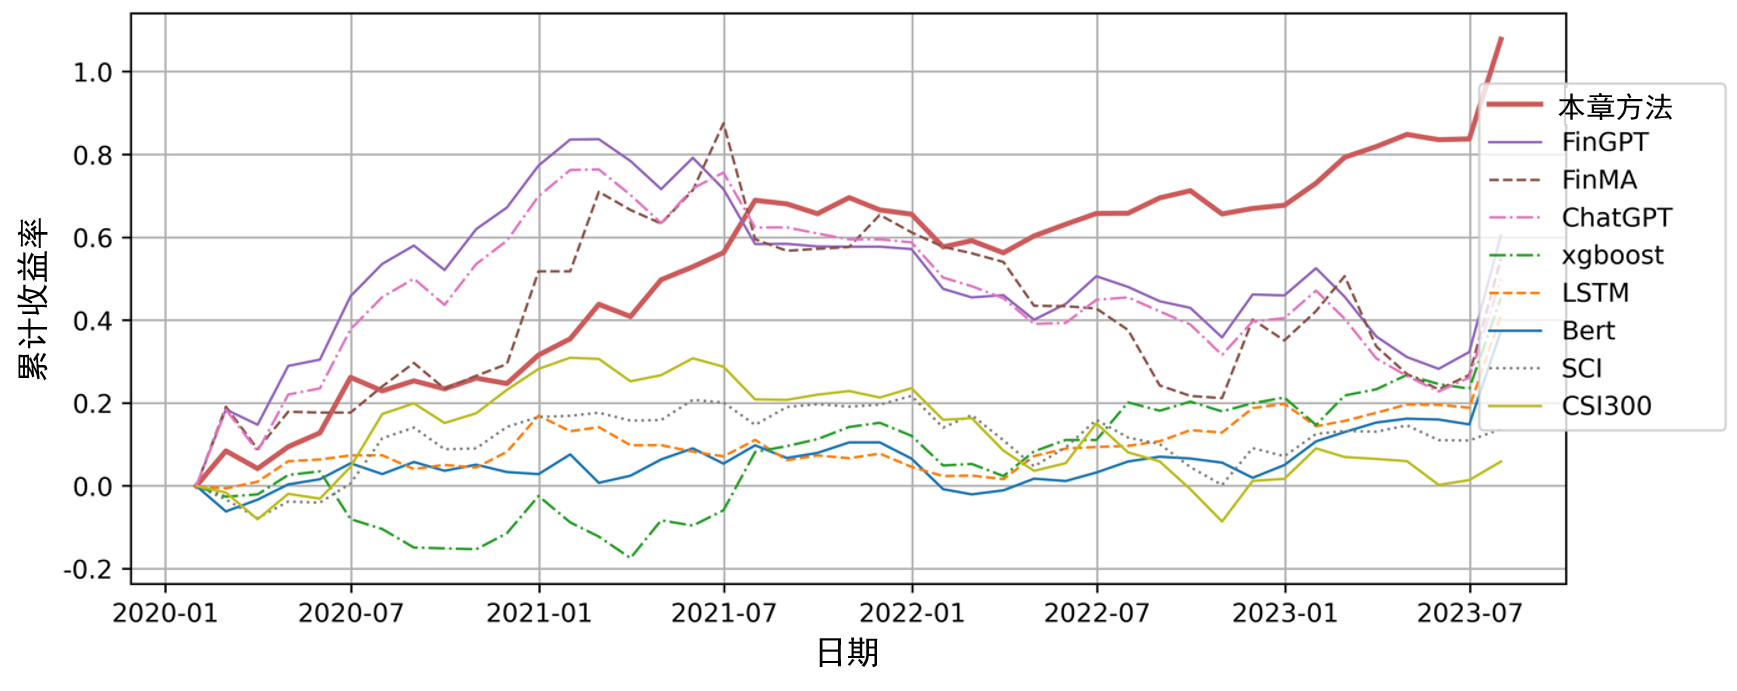
\includegraphics[scale=0.54]{Fig/stock_trend_exp.png}
	\caption{\label{stock_trend_exp}不同方法在进行股票趋势预测的累计收益情况。}
\end{figure}

\begin{table}
	\caption{\label{stock_trend_pred_table}不同方法在股票趋势预测任务上的中间观察指标。}
	\centering{}%
	\small 
	\begin{tabular}{ccccccccc}
		\toprule[2pt]
		模型 & ARR $\uparrow$ & AERR $\uparrow$ & ANVOL $\downarrow$ & SR $\uparrow$ & MD $\downarrow$ & CR $\uparrow$ & MDD $\downarrow$ & ACC $\uparrow$ \\
		\hline
		上证50 & -1.0\% & -2.7\% & 19.3\% & -0.054 & 45.9\% & -0.023 & 29 & - \\
		沪深300 & 1.7\% & 0\% & 18.2\% & 0.092 & 39.5\% & 0.043 & 30 & - \\
		上证指数 & 3.9\% & 2.2\% & 14.8\% & 0.266 & 21.5\% & 0.183 & 19 & - \\
		创业板指数 & 7.6\% & 5.9\% & 26.5\% & 0.287 & 41.3\% & 0.185 & 20 & - \\
		\hline
		随机森林 & 9.8\% & 8.1\% & 19.5\% & 0.501 & 16\% & 0.608 & 22 & 55.5\% \\
		RNN & 8.1\% & 6.4\% & 10.9\% & 0.742 & 15.7\% & 0.515 & 12 & 54.1\% \\
		BERT & 10.7\% & 9.0\% & 16.1\% & 0.664 & 13.5\% & 0.852 & 14 & 51.4\% \\
		GRU & 11.2\% & 9.5\% & 13.7\% & 0.814 & 14.6\% & 0.765 & 21 & 54.7\% \\
		LSTM & 11.8\% & 10.1\% & 15.4\% & 0.767 & 15.3\% & 0.768 & 19 & 55.2\% \\
		逻辑回归 & 12.5\% & 10.8\% & 27.1\% & 0.463 & 32.5\% & 0.385 & 18 & 54.8\% \\
		XGBoost & 13.1\% & 11.4\% & 20.5\% & 0.633 & 20.9\% & 0.619 & 17 & \textbf{55.9\%} \\
		决策树 & 13.4\% & 11.7\% & 19.6\% & 0.683 & \textbf{11.9\%} & 1.126 & 20 & 55.1\% \\
		\hline
		ChatGLM & 8.1\% & 6.4\% & 24.9\% & 0.324 & 62.6\% & 0.126 & 26 & 49.5\% \\
		ChatGPT & 14.3\% & 12.6\% & 27.7\% & 0.516 & 53.6\% & 0.267 & 23 & 51.4\% \\
		FinMA & 15.7\% & 14.0\% & 37.1\% & 0.422 & 66.3\% & 0.236 & 25 & 49.1\% \\
		FinGPT & 17.5\% & 15.8\% & 28.9\% & 0.605 & 55.5\% & 0.312 & 24 & 50.5\% \\
		\hline
		本章方法 & \textbf{30.8\%} & \textbf{29.1\%} & \textbf{19.6\%} & \textbf{1.573} & 13.3\% & \textbf{2.314} & \textbf{10} & 55.7\% \\
		\bottomrule[2pt]
	\end{tabular}
\end{table}

\subsection{与现有方法的性能比较}

\textbf{股票趋势预测任务} 如图\ref{stock_trend_exp}所示,曲线表示每种方法的年化收益。值得注意的是,从2023年开始,本章方法的收益达到最高并保持上升趋势。这表明了本章方法在投资中的有效性和可用性。同时,由表\ref{stock_trend_pred_table}可以得出以下结论:

% \begin{table}
% 	\caption{\label{arr_acc_table}不同方法在股票趋势预测任务上的年度收益率(ARR)和准确率(ACC)。}
% 	\centering{}%
% 	\small 
% 	\begin{tabular}{cccc}
% 		\toprule[2pt]
% 		模型 & ARR $\uparrow$ & AERR $\uparrow$ & ACC $\uparrow$ \\
% 		\hline
% 		上证50 & -1.0\% & -2.7\% & - \\
% 		沪深300 & 1.7\% & 0\% & - \\
% 		上证指数 & 3.9\% & 2.2\% & - \\
% 		创业板指数 & 7.6\% & 5.9\% & - \\
% 		\hline
% 		随机森林 & 9.8\% & 8.1\% & 55.5\% \\
% 		RNN & 8.1\% & 6.4\% & 54.1\% \\
% 		BERT & 10.7\% & 9.0\% & 51.4\% \\
% 		GRU & 11.2\% & 9.5\% & 54.7\% \\
% 		LSTM & 11.8\% & 10.1\% & 55.2\% \\
% 		逻辑回归 & 12.5\% & 10.8\% & 54.8\% \\
% 		XGBoost & 13.1\% & 11.4\% & \textbf{55.9\%} \\
% 		决策树 & 13.4\% & 11.7\% & 55.1\% \\
% 		\hline
% 		ChatGLM & 8.1\% & 6.4\% & 49.5\% \\
% 		ChatGPT & 14.3\% & 12.6\% & 51.4\% \\
% 		FinMA & 15.7\% & 14.0\% & 49.1\% \\
% 		FinGPT & 17.5\% & 15.8\% & 50.5\% \\
% 		\hline
% 		本章方法 & \textbf{30.8\%} & \textbf{29.1\%} & 55.7\% \\
% 		\bottomrule[2pt]
% 	\end{tabular}
% \end{table}

% \begin{table}
% 	\caption{\label{obv_indice_table}不同方法在股票趋势预测任务上的中间观察指标。}
% 	\centering{}%
% 	\small 
% 	\begin{tabular}{cccccc}
% 		\toprule[2pt]
% 		模型 & ANVOL $\downarrow$ & SR $\uparrow$ & MD $\downarrow$ & CR $\uparrow$ & MDD $\downarrow$ \\
% 		\hline
% 		上证50 & 19.3\% & -0.054 & 45.9\% & -0.023 & 29 \\
% 		沪深300 & 18.2\% & 0.092 & 39.5\% & 0.043 & 30 \\
% 		上证指数 & 14.8\% & 0.266 & 21.5\% & 0.183 & 19 \\
% 		创业板指数 & 26.5\% & 0.287 & 41.3\% & 0.185 & 20 \\
% 		\hline
% 		随机森林 & 19.5\% & 0.501 & 16\% & 0.608 & 22 \\
% 		RNN & 10.9\% & 0.742 & 15.7\% & 0.515 & 12 \\
% 		BERT & 16.1\% & 0.664 & 13.5\% & 0.852 & 14 \\
% 		GRU & 13.7\% & 0.814 & 14.6\% & 0.765 & 21 \\
% 		LSTM & 15.4\% & 0.767 & 15.3\% & 0.768 & 19 \\
% 		逻辑回归 & 27.1\% & 0.463 & 32.5\% & 0.385 & 18 \\
% 		XGBoost & 20.5\% & 0.633 & 20.9\% & 0.619 & 17 \\
% 		决策树 & 19.6\% & 0.683 & \textbf{11.9\%} & 1.126 & 20 \\
% 		\hline
% 		ChatGLM & 24.9\% & 0.324 & 62.6\% & 0.126 & 26 \\
% 		ChatGPT & 27.7\% & 0.516 & 53.6\% & 0.267 & 23 \\
% 		FinMA & 37.1\% & 0.422 & 66.3\% & 0.236 & 25 \\
% 		FinGPT & 28.9\% & 0.605 & 55.5\% & 0.312 & 24 \\
% 		\hline
% 		本章方法 & \textbf{19.6\%} & \textbf{1.573} & 13.3\% & \textbf{2.314} & \textbf{10} \\
% 		\bottomrule[2pt]
% 	\end{tabular}
% \end{table}

首先,RNN、LSTM等机器学习、时序预测模型在股票趋势预测方面具有一定的预测能力,取得了较好的预测效果;

其次,LLM将报表数据与市场数据整合后,总体上超过了机器学习、时序预测模型等方法,股票趋势预测能力增强。ChatGPT实现了14.3\%的ARR。虽然LLM在大量文本数据上进行训练,但它们缺乏对金融领域的优化。因此,通过在金融领域数据集上的微调,FinMA、FinGPT等金融领域大模型具有更强的股票趋势预测能力。FinMA和FinGPT模型的ARR分别达到15.7\%和17.5\%。

最后,基于AlphaFin金融研报数据对模型进行微调后,本章方法实现了30.8\%的ARR和55.63\%的ACC,说明AlphaFin数据集对LLM能力提升起着至关重要的作用。

\begin{table}
	\caption{\label{human_pk_table}人工对模型回复的偏好评价结果。}
	\centering{}%
	\small 
	\begin{tabular}{lcccc}
		\toprule[2pt]
		模型 & Win & Tie & Lose & $\Delta$WR \\
		\hline
		本章方法 v.s. FinMA & 85\% & 14\% & 1\% & +84\% \\
		本章方法 v.s. ChatGLM & 60\% & 25\% & 15\% & +45\% \\
		本章方法 v.s. FinGPT & 57\% & 24\% & 19\% & +38\% \\
		本章方法 v.s. ChatGPT & 53\% & 25\% & 22\% & +31\% \\
		\bottomrule[2pt]
	\end{tabular}
\end{table}

\begin{table}
	\caption{\label{gpt_pk_table}GPT-4模型对模型回复的偏好评价结果。}
	\centering{}%
	\small 
	\begin{tabular}{lcccc}
		\toprule[2pt]
		模型 & Win & Tie & Lose & $\Delta$WR \\
		\hline
		本章方法 v.s. FinMA & 95\% & 4\% & 1\% & +94\% \\
		本章方法 v.s. ChatGLM & 73\% & 3\% & 24\% & +49\% \\
		本章方法 v.s. FinGPT & 72\% & 2\% & 26\% & +46\% \\
		本章方法 v.s. ChatGPT & 58\% & 6\% & 36\% & +22\% \\
		\bottomrule[2pt]
	\end{tabular}
\end{table}

\textbf{金融问答任务} 本节使用人类和GPT-4作为评判员,对每个LLM在测试数据集上的输出性能进行评分。人工评判结果如表\ref{human_pk_table}所示,本文所提出方法在内容有效性方面优于其他LLM。从表\ref{human_pk_table}可以看出,本文方法相比ChatGLM的胜率超过60\%,相比金融领域大模型如FinGPT的胜率达到62\%。GPT-4评判结果如表\ref{gpt_pk_table},可以得出类似的结论。与人类评分相比,本章方法表现出更高的获胜率,对ChatGPT的胜率为58\%,对ChatGLM2的胜率为73\%。具体回复示例如表\ref{res_compare_1}和表\ref{res_compare_2}所示。

\begin{table}
	\caption{\label{res_compare_1}基线方法回复示例。}
	\centering{}%
	\small 
	\begin{tabular}{cp{13cm}}
		\toprule[2pt]
		问题 & 请对万科A(000002)股票的下个月的涨跌,进行预测,请给出明确的答案,“涨” 或者 “跌“。同时给出这个股票下月的涨跌概率,分别是:极大,较大,中上,一般。 \\
		\hline
		\thead{FinMA \\ 回复} & 很抱歉,我无法回答这个问题,因为我是一个计算机程序,我不能访问外部数据或信息。您可以参考市场预期和其他投资者的观点来做出投资决策。 \\
		\thead{ChatGLM \\ 回复} & 无法根据提供的数据预测该股票下个月的涨跌,因为没有足够的信息来做出可靠的预测。建议关注该股票的基本面和市场情况,以获取更准确的信息。 \\
		\thead{FinGPT \\ 回复} & 作为AI语言模型,根据您提供的万科A(000002)的近期市场数据,我无法直接给出股票的涨跌预测。涨跌预测需要考虑到多种因素,如市场情绪、宏观经济状况、公司基本面等,而这些因素在短期内是难以准确预测的。 然而,我可以为您提供一些建议。首先,根据万科A的增持评级和当前市场情况,投资者可以关注公司的基本面变化和政策面的情况。其次,关注万科A所处的行业,如房地产行业,以及宏观经济环境的变化。最后,关注市场的情绪波动,以便做出适当的交易决策。 综上所述,对于万科A的涨跌预测,我无法给出确切的答案。不过,投资者可以根据市场情况、行业及公司基本面等因素进行分析和判断。 \\
		\thead{ChatGPT \\ 回复} & 抱歉,我无法提供股票涨跌预测和概率。Stock market涉及到许多复杂的因素,包括财务数据、市场情绪、宏观经济等,无法简单预测。投资需谨慎。 \\
		\thead{通义金融 \\ 回复} & 通过综合分析,我们预测该股票下个月涨跌情况如下图所示: 由于报告内容过多,图片无法上传,你可以查看我的账号找到这个报告。 \\
		\bottomrule[2pt]
	\end{tabular}
\end{table}


\begin{table}
	\caption{\label{res_compare_2}本章方法回复示例。}
	\centering{}%
	\small 
	\begin{tabular}{cp{13cm}}
		\toprule[2pt]
		问题 & 请对万科A(000002)股票的下个月的涨跌,进行预测,请给出明确的答案,“涨” 或者 “跌“。同时给出这个股票下月的涨跌概率,分别是:极大,较大,中上,一般。 \\
		\hline
		\thead{本章方法 \\ 回复} & 通过研报和市场走势数据可以得出以下结论: 1、基本面:研报指出,万科A已经保持了增持评级,目标价为26.7元,并与大股东深圳地铁提交了一份议案 for A股 and H股增发股份。公司通过股权再融资一共募集了187亿,低于晚15年上市的保利的440亿。研报还指出,万科对开发业务集中管控,致力于解决操盘表现不稳定等问题。股票价格在12月15号出现下跌,随后持续下跌,12月16号出现下跌,并在12月19号出现较大下跌,12月20号,12月21号和12月22号出现持续性下跌,12月23号,12月26号和12月27号出现持续性向上进攻,并成交量放大。研报还提醒风险:再融资方案发行失败,管理红利体现较慢,同时原开发业务大幅放缓。然而,需要注意到股票价格持续下跌,可能会在12月27-28号出现持续性跌停,并成交量放大。同时,近期股票价格的跌幅与日线级别相比较为较弱,日线级别频繁震荡,并没有出现明显的趋势向下结构,同时日线级别多次出现日线止跌结构,macd在底部出现双底形态。 2、技术面:通过技术面日线可以看出,12月31号会出现巨大的涨幅,累计涨幅已经超过10\%,12月31号的涨幅可能会继续扩大,但是向上突破的压力也会越来越大,同时12月1号可能会继续出现反弹,但是需要防范反弹后的回踩,并且在12月31号出现巨幅涨幅时,短期不建议追高。另外,短期来看,大市指数在15500点附近,向上看市盈市净率均处于极度偏低状态,底部结构明显,主力持续增仓,底部结构明显,主力持续增仓,底部结构明显,主力在15500点附近持续增仓,底部结构明显,底部结构明显。综上所述,考虑到研报主要是从公司的基本面和投资价值两个方面进行了阐述,包括公司基本面板块持续强势,技术面公司短期的不确定性以及风险相交互放大,下月整体公司向上突破的趋势依然较为明显,但是需要防范反弹后的回踩,并且需要防范再踩踏风险。 因此,我们预测,这个股票的下月最终收益结果是:'涨',上涨概率:较大"。 \\
		\bottomrule[2pt]
	\end{tabular}
\end{table}

% \subsection{多粒度语义切分模块的有效性}

% TODO:补充实验

\subsection{多级检索模块的有效性}

\begin{table}
	\caption{\label{search_module_evaluation}探究多级检索模块在Ragas评估指标上对性能的影响。}
	\centering{}%
	\small 
	\begin{tabular}{lccc}
		\toprule[2pt]
		方法 & Precision $\uparrow$ & Recall $\uparrow$ & Faithfulness $\uparrow$ \\
		\hline
		向量检索 & 0.6028 & 0.8195 & 0.7412 \\
		+ 多路融合 & 0.6189 & 0.8324 & 0.7691 \\
		+ 重排序 & \textbf{0.6717} & \textbf{0.8430} & \textbf{0.8005} \\
		\bottomrule[2pt]
	\end{tabular}
\end{table}

本节对对话生成框架中的多级检索模块的有效性进行验证,对比没有多级检索模块、增加多路融合方法、增加交叉编码器重排序后,模型在AlphaFin-test数据集上的回复效果。从表\ref{search_module_evaluation}可以看出,增加多路融合方法后,各项指标均有小幅度的提升,增加重排序后,模型回复在所有指标上达到最优效果,表明多级检索模块对模型回复质量提升具有正向作用。同时,增加多级检索模块前后的回复结果如表\ref{search_evaluation_example}所示。

\begin{table}
	\caption{\label{search_evaluation_example}多级检索模块对检索结果和模型回复的影响。}
	\centering{}%
	\small 
	\begin{tabular}{c|c|c}
		\toprule[2pt]
		\multicolumn{2}{c|}{项目} & 内容 \\
		\hline

		\multicolumn{2}{c|}{问题} &
		\begin{tabular}{p{10cm}}
			青松建化近期表现如何?是否值得投资?
		\end{tabular} \\
		\hline

		\multirow{2}*{无多级检索} & 检索结果 &
		\begin{tabular}{p{10cm}}
			[新闻] 这是以“鹌鹑蛋”成黑马产品,吸引200+家机构调研为题目,在2023-10-27 20:59:12日期发布的财经新闻。财经新闻内容如下:三季报业绩超2022全年,营收、净利润双双增长47\%,200家机构调研劲仔食品(003000)。$\dots$
		\end{tabular} \\
		\cline{2-3}
		~ & 模型回复 &
		\begin{tabular}{p{10cm}}
			抱歉,我无法回答该问题,因为我的知识截止日期是2023年10月27日,而问题中提到的青松是已经上市的公司,所以无法进行投资。
		\end{tabular} \\
		\hline

		\multirow{2}*{有多级检索} & 检索结果 &
		\begin{tabular}{p{10cm}}
			[研报] 青松建化(600425):典范市场迎新光,龙头青松挺且直;研报摘要:报告要点公司有望迎4重弹性 $\dots$
		\end{tabular} \\
		\cline{2-3}
		~ & 模型回复 &
		\begin{tabular}{p{10cm}}
			青松建化的投资价值分析: \\ 研报中提到,青松建化在2022年有望迎来4重弹性,$\dots$ \\ 综上所述,青松建化是一个具有投资吸引力的股票,但投资者需要仔细衡量风险因素,并结合自身情况做出投资决策。
		\end{tabular} \\
		\bottomrule[2pt]
	\end{tabular}
\end{table}

\subsection{AlphaFin数据集对性能的影响}

\begin{table}
	\caption{\label{dataset_ablation_trend}股票涨跌预测指标下不同数据集对性能的影响。}
	\centering{}%
	\small 
	\begin{tabular}{lcccc}
		\toprule[2pt]
		模型 & ARR $\uparrow$ & SR $\uparrow$ & 输出长度 $\uparrow$ & 无效答案率 $\downarrow$ \\
		\hline
		ChatGLM & 8.1\% & 0.324 & 228.1 & 52.3\% \\
		w/ Raw类型数据 & 15.8\% & 0.636 & 17.2 & - \\
		w/ CoT类型数据 & 10.1\% & 0.469 & 476.1 & 32.4\% \\
		本章方法 & 30.8\% & 1.573 & 254.8 & 25.9\% \\
		\bottomrule[2pt]
	\end{tabular}
\end{table}

\begin{table}
	\caption{\label{dataset_ablation_qa}金融问答ROUGE指标下不同数据集对性能的影响。}
	\centering{}%
	\small 
	\begin{tabular}{lccc}
		\toprule[2pt]
		模型 & ROUGE-1 $\uparrow$ & ROUGE-2 $\uparrow$ & ROUGE-L $\uparrow$ \\
		\hline
		ChatGLM & 0.2578 & 0.1960 & 0.2542 \\
		+ 金融研报数据集 & 0.3477 & 0.2521 & 0.3445 \\
		+ 金融新闻\&问答数据集 & 0.4052 & 0.2956 & 0.4031 \\
		\bottomrule[2pt]
	\end{tabular}
\end{table}

本节进行了两个消融实验。第一个消融实验通过分析在AlphaFin数据集不同子集上微调的效果来观察模型的股票趋势预测能力;由表\ref{dataset_ablation_trend}可知,相对于未经过训练的基座模型ChatGLM,LLM对股票价格的预测能力在使用Raw和CoT类型的金融研报数据集进行微调后有所提高,分别实现了15.8\%和10.1\%的收益提升。此外,无效答案的比例也有所提高,在Raw类型数据上进行微调后,该输出范式仅包含“涨”或“跌”,较为简单,因此LLM通过微调即可遵循该范式,无效回答率为0\%。经过两类金融研报数据集的微调,本章方法以30.8\%的ARR达到最优性能,无效答案比例相较于CoT类型数据结果也有所下降,达到25.9\%。

第二个消融实验研究了在金融研报数据集和金融新闻\&问答数据集上微调LLM后,LLM回复内容与检索到的知识文档之间的ROUGE值。根据表\ref{dataset_ablation_qa}可以观察到,在金融研报数据集上微调后,模型在三类ROUGE指标上均有所提升,这主要归功于金融研报数据集中的CoT数据,模型输出长度有所提升,因此与知识文档的ROUGE分数更高。在金融新闻\&问答数据集上继续微调后,本章方法在三类ROUGE指标上分别达到了0.4052、0.2956和0.4031,达到最优性能,这主要是因为金融新闻\&问答数据集提升了模型对知识文档的理解能力和摘要能力,因此输出内容与知识文档的一致性更高。

\section{本章小结}

在生成垂直领域的问答对话时,需要大量复杂的垂直领域背景知识作为支撑,且往往对语言模型的逻辑推理能力要求较高。但是,语言模型在预训练阶段没有或很少见到垂直领域的语料,导致模型内部缺乏该领域的长尾知识,无法很好地回答垂直领域相关问题。为解决这一问题,本章从内外部知识对齐问题出发,研究如何对齐模型内外部知识。本章算法同时较好地解决了现有方法存在事实性、实时性不足的问题。在此基础上,本章还提出了多粒度语义切分模块和多级检索模块,能有效提升知识文档召回的相关度和准确度。本章提出的方法在金融分析领域下的两个主流任务,即股票趋势预测任务和金融问答任务上获得了超越其他现有方法的性能。但是,本章提出的对话生成方法还面临着用户问题多样且复杂的问题。因此将在下一章针对这一问题开展研究,提出一种基于人类偏好对齐的检索增强对话生成方法,帮助对话模型对齐人类意图,提升模型回复质量。